\chapter{操作系统的组织结构}\label{ch02}

操作系统的一个核心需求是同时支持多个活动。
例如,使用\autoref{ch01}中介绍的系统调用,一个进程可以通过\texttt{fork}创建新的进程。
操作系统必须在进程之间\emph{分时共享(time-share)}计算机的资源。
例如,即使有比硬件处理器数量更多的进程,操作系统也要保证所有的进程都能获得执行的机会。
操作系统还必须实现进程之间的\emph{隔离(isolation)}。
即,如果一个进程有bug并且失败了,它不应该影响到那些不依赖这个进程的进程。
然而,完全的隔离太过苛刻,因为进程之间可能需要交互,管道就是一个例子。
因此一个操作系统必须满足这三个要求:多路复用,隔离性,交互性。

这一章提供了操作系统是如何组织以满足三个需求的概述。
事实证明有很多方法可以做到这一点,但本文专注于基于\emph{宏内核(monolithic kernel)}的主流设计,很多Unix操作系统都采用了宏内核的方式。
本章还提供了xv6进程的概述和当xv6启动时第一个进程的创建,进程是xv6中的隔离单元。

xv6运行在一台\emph{多核(multi-core)}\footnote{本书中的“多核”指的是共享内存但可以并行执行的多个CPU,每一个都有自己的寄存器。本书有时也会用术语\emph{多处理器(multiprocessor)}作为多核的同义词,尽管多处理器也可以指代有多个处理器芯片的计算机。}  RISC-V微处理器上,很多底层设施(例如,进程的实现)是RISC-V特定的。
RISC-V是64位的CPU,xv6也是用“LP64”C写成的,“LP64”的意思C语言中的是long(L)和pointer(P)都是64位的,而int是32位的。
这本书假设读者已经了解了某些架构的机器级编程,并在遇到时介绍RISC-V规范的思路。
RISC-V的一份很有用的参考文献是“The RISC-V Reader: An Open Architecture Atlas”[15]。
用户级的ISA[2]和特权架构[3]都是官方的规范。

一台完整计算机中的CPU被支持硬件环绕,它们中的大多数组成了I/O接口。
xv6的支持硬件通过qemu的“-machine virt”选项进行模拟。
其中包括RAM,一个包含启动代码的ROM,一个连接到用户键盘/屏幕的串口,一个用于存储的磁盘。

\section{抽象物理资源}
说到操作系统,很多人的第一个问题可能是为什么需要它?
事实上,我们可以把\autoref{t0-1}中的系统调用实现为库,然后让应用链接它。
在这种模式下,每一个应用甚至可以有根据自己需求量身定做的库。
应用可以直接和硬件资源交互,并且采用对应用来说最合适的方式来使用资源(例如,用来实现很高或者可预测的性能)。
一些嵌入式设备或实时系统的操作系统就是以这种方式组织的。

这种库方式的缺点是,如果有不止一个应用在运行,那么这些应用必须行为良好。
例如,每一个应用必须周期性地放弃处理器,这样其他应用才能运行。
如果所有的应用都互相信任并且没有bug,那么这种\emph{协作(co-operative)}分时方案可能也OK。
然而,更常见的情况是应用并不信任彼此,并且还可能有bug,因此我们通常需要比协作方案更强的隔离性。

为了实现强隔离性,禁止应用直接访问敏感的硬件资源,而是将资源抽象为服务会很有帮助。
例如,应用和文件系统交互时通过\texttt{open, read, write, close}系统调用,而不是读写原始的磁盘扇区。
这为应用程序提供了路径名的便利,并且允许操作系统(作为接口的实现者)来管理磁盘。

与此类似,Unix在进程之间透明地切换处理器,必要时保存并恢复寄存器状态,因此应用不需要考虑时间共享。
这种透明性允许操作系统即使遇到一些陷入无限循环的应用时也可以共享处理器。

作为另一个例子,Unix进程使用\texttt{exec}来构建自己的内存镜像,而不是直接和物理内存交互。
这允许操作系统来决定把进程加载到内存的哪一部分;如果内存很紧张,操作系统甚至可以把进程的部分数据存储在磁盘上。
\texttt{exec}也为应用提供了把可执行程序镜像存储在文件系统中的便利。

Unix进程之间的很多交互方式都是通过文件描述符。
文件描述符不仅仅通过抽象消除了一些细节(例如,管道或文件中的数据存储在哪里),它们还定义了一种简化交互的方式。
例如,如果一个管道中的某个应用失败了,那么内核会为管道中的下一个进程生成end-of-file。

如你所见,\autoref{t0-1}中的系统调用接口被精心设计,以在给程序员提供便利的同时提供强隔离性。
Unix接口不是唯一抽象资源的方式,但它被证明是一种非常优秀的方式。

\section{用户模式、内核模式、系统调用}
强隔离性需要应用和操作系统之间有明显的界限。
如果一个应用失败了,我们不想让操作系统或者其他应用也失败。
反而,操作系统应该能清理失败的应用,然后继续运行其他的应用。
为了达到强隔离性,操作系统必须保证应用不能修改(或者甚至不能读取)操作系统的数据结构和指令,也不能访问其他进程的内存。

处理器为强隔离性提供了硬件支持。
例如,x86处理器和很多其他处理器一样,有两种执行指令的模式:\emph{内核模式(kernel mode)和\emph{用户模式(user mode)}}。
在内核模式下,处理器被允许执行\emph{特权指令(privileged instruction)}。
例如,读写磁盘(或者其他I/O设备)就涉及到特权指令。
如果一个用户模式的应用尝试执行一条特权指令,那么处理器并不会执行这条指令,但会切换到内核模式,这样内核模式的程序可以清理掉这个应用,因为它做了它不该做的。
第0章中的\autoref{f0-1}展示了这个过程。
一个用户模式的应用只能执行用户模式的指令(例如,数字相加),并且在\emph{用户空间(user space)}运行,而内核模式的应用还可以执行特权指令,并且在\emph{内核空间(kernel space)}运行。
在内核空间中(或者在内核模式下)运行的程序被称为\emph{内核(kernel)}。

如果一个应用想要读取或写入一个磁盘上的文件,那么它必须过渡到内核来做这件事,因为应用自身不能执行I/O指令。
处理器提供了特殊的指令用于将处理器从用户模式转换到内核模式,并且在内核指定的入口点进入内核。(x86处理器提供了\texttt{int}指令来实现这一点。)
一旦处理器切换到内核模式,内核可以验证系统调用的参数,决定应用是否被允许执行请求的操作,然后拒绝它或者执行它。
过渡时的入口点是内核设置的,这一点非常重要;如果应用可以决定内核的入口点,一个恶意的应用就可以在一个跳过参数验证的地方进入内核。

\section{内核架构}
一个关键的设计问题就是操作系统的哪些部分应该在内核态运行。一种可能是整个操作系统都在内核里运行,这样所有系统调用的实现就都在内核态运行。这种架构被称为\emph{宏内核(monolithic kernel)}。

在这种架构下整个操作系统都在有完全的硬件特权的情况下运行。这种架构非常方便,因为操作系统的设计者们不需要决定操作系统的哪些部分不需要完全的硬件特权。不仅如此,它还有利于操作系统不同模块之间的协作。例如,操作系统可以拥有一个由文件系统和虚拟内存系统所共享的缓冲区缓存。

宏内核架构的缺点是操作系统的不同部分之间的接口通常很复杂(正如我们将在之后看到的),而且也因此很容易导致操作系统开发者犯错。在宏内核中错误是致命的,因为一个内核模式下的错误通常导致整个内核的终止。如果内核终止了,计算机就会停止工作,因此所有的应用也会终止。计算机必须重启才能再次工作。

为了减少内核中错误的风险,OS的设计者们可以最小化在内核态中运行的操作系统代码的数量,并在用户态下执行操作系统的大部分内容。这种内核架构被称为\emph{微内核(micro kernel)}。

\autoref{f2-1}展示了微内核的设计。图中文件系统作为用户级进程运行。以进程的形式运行的OS服务被称为server。为了允许应用和文件server交互,内核会提供一种进程间的通信机制来允许一个用户态的进程向另一个进程发送消息。例如,如果一个应用例如shell想要读写一个文件,它会向文件server发送一条消息然后等待响应。

\begin{figure}[htbp]
    \centering
    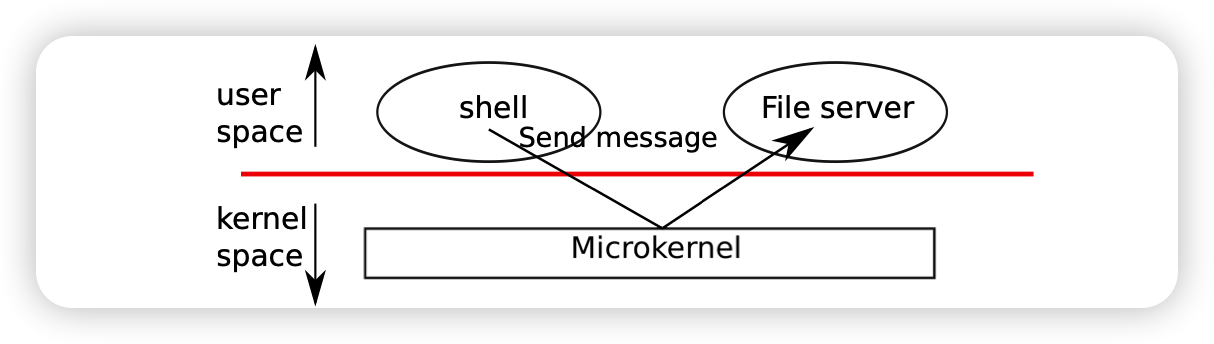
\includegraphics[width=0.8\textwidth]{../imgs/f2-1.png}
    \caption{有一个文件server的微内核}
    \label{f2-1}
\end{figure}

在微内核中,内核的接口由一些底层的函数,例如启动应用、发送消息、访问设备硬件等等,组合而成。这种架构会让内核变得相对简单一点,因为操作系统的大部分都在用户态的server中运行。

Xv6和大多数Unix操作系统一样被实现为宏内核。因此,在xv6中,内核接口也对应着操作系统接口,内核实现了全部的操作系统。因为xv6并不提供很多服务,因此它的内核比一些微内核还要小。

\section{进程概览}
Xv6中的隔离单元(和其他Unix操作系统一样)是\emph{进程(process)}。进程的抽象可以阻止一个进程破坏或者窥探另一个进程的内存、CPU、文件描述符等内容。它还可以防止一个进程破坏内核本身,因此一个进程不可能颠覆内核的隔离机制。内核必须小心实现进程的抽象,因为一个有bug的或者恶意的应用可能会欺骗内核或硬件做一些坏事(例如规避强制隔离)。内核用来实现进程的机制包括用户态/内核态标志、地址空间和线程的时间分片。

为了实现强制隔离,进程抽象为每个程序提供了它有一台自己的私有机器的假象。一个进程给一个程序提供了看似私有的内存系统、或者说\emph{地址空间(address space)},其他进程不能读取或写入。一个进程还为程序提供了看似独占的CPU来执行程序的指令。

Xv6使用页表(由硬件实现)为每个进程提供私有的地址空间。x86的页表把一个\emph{虚拟地址(virtual address)}(x86指令中操作的地址)翻译(或者说“映射”)到一个\emph{物理地址(physical address)}(处理器芯片送到主存的地址)。

Xv6为每个进程维护了一个单独的页表,它定义了进程的地址空间。如\autoref{f2-2}所示,一个地址空间包含了进程的\emph{用户内存(user memory)},它从虚拟地址0处开始。首先是指令,接是全局变量、然后是栈,最后是一个进程可以按需扩张的“堆”区域(用于malloc)。

\begin{figure}[htbp]
    \centering
    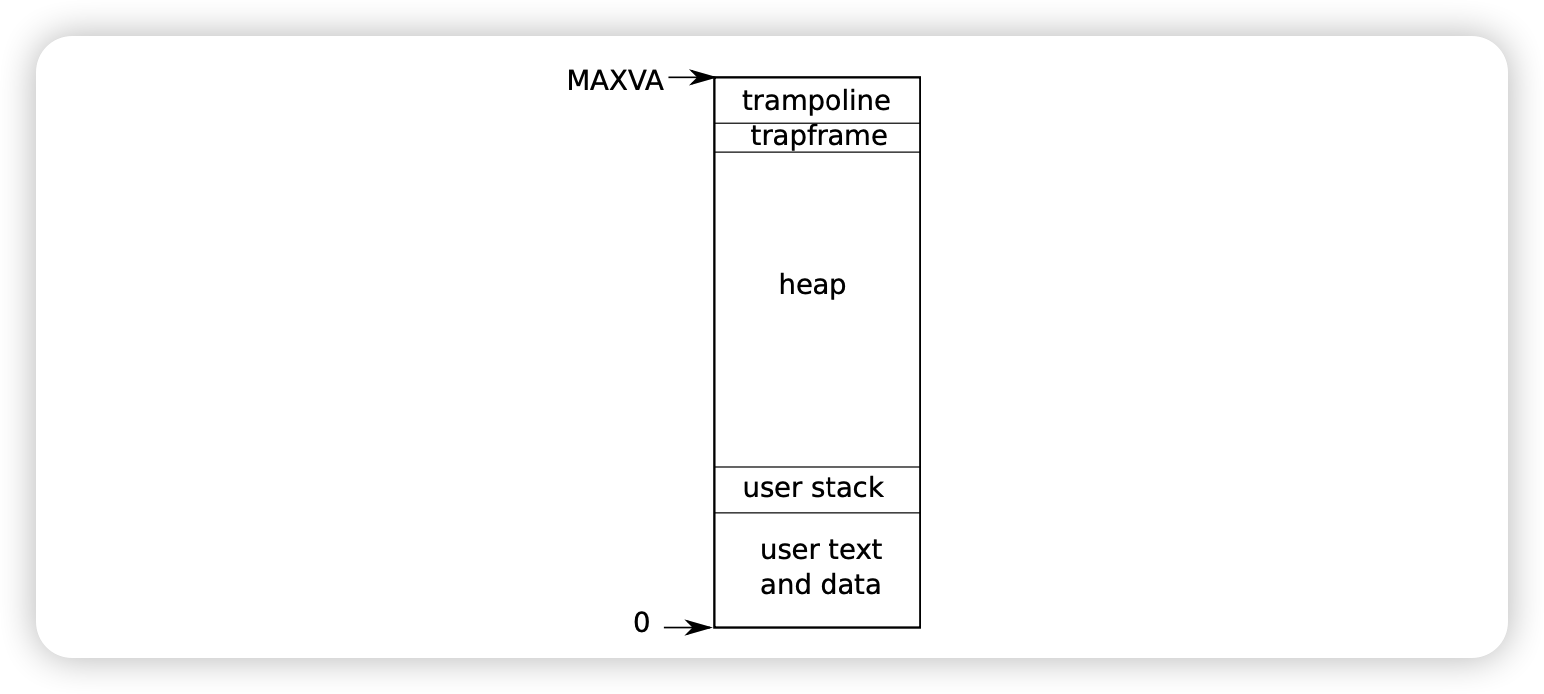
\includegraphics[width=0.8\textwidth]{../imgs/f2-2.png}
    \caption{虚拟地址空间的布局}
    \label{f2-2}
\end{figure}

每个进程的地址空间都把内核的指令和数据也映射到用户程序的内存中。当一个进程触发一个系统调用时,系统调用会在进程的地址空间的内核映射中执行。这样安排是为了让内核的系统调用代码能直接访问用户内存。为了给用户内存留出充足的空间,xv6的地址空间在高地址处映射内核,从\texttt{0x80100000}开始。

\begin{figure}[htbp]
    \centering
    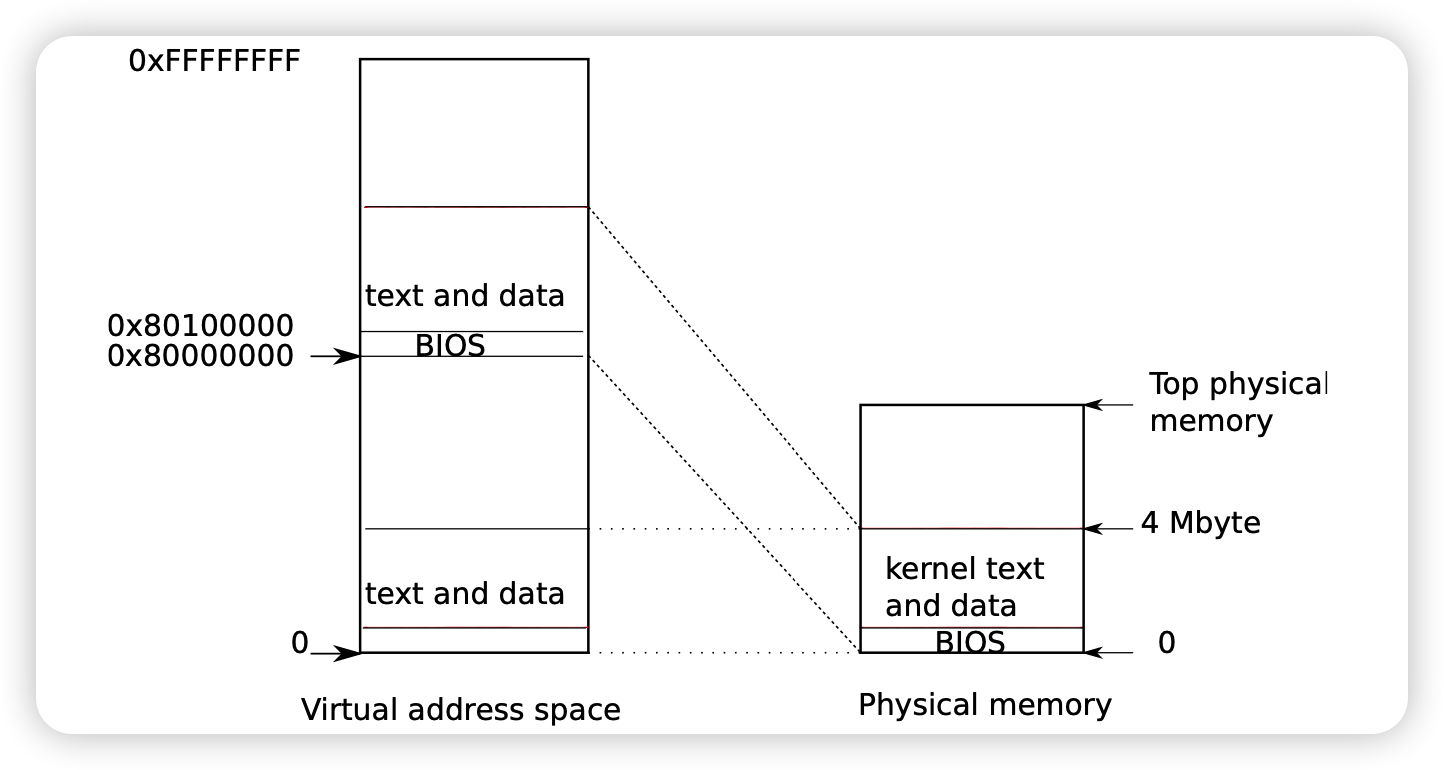
\includegraphics[width=0.8\textwidth]{../imgs/f2-3.png}
    \caption{虚拟地址空间的布局}
    \label{f2-3}
\end{figure}

Xv6的内核为每个进程维护很多状态,都存储在一个\texttt{struct proc}里(2337)。一个进程中最重要的内核状态是它的页表、内核栈和运行状态。我们将使用记号\texttt{p->xxx}来引用\texttt{proc}结构体的元素。

每个进程都有一个执行线程(或者简称\emph{线程(thread)})来执行进程的指令。一个线程可以被挂起之后再恢复。为了在进程间透明地切换,内核会挂起当前正在执行的线程然后恢复另一个进程的线程。一个线程的很多状态(局部变量、函数调用的返回地址)都存储在线程的栈中。每个进程都有两个栈:一个用户栈和一个内核栈(\texttt{p->kstack})。当进程在执行用户指令时,只会用到它的用户栈,它的内核栈是空的。当进程进入内核时(因为一次系统调用或者中断),内核代码会在进程的内核栈上执行;然而当一个进程在内核中时,它的用户栈仍然包含保存的数据,但并不会被积极使用。一个进程的线程在积极使用其用户栈和内核栈之间交替。内核栈是独立的(并且被保护不受用户代码的影响)因此即使进程破坏了它的用户栈,内核也可以继续执行。

当一个进程进行系统调用时,处理器会切换到内核栈、提高硬件的权限级别,并开始执行实现了系统调用的内核指令。当系统调用结束时,内核会返回到用户空间:硬件会降低权限级别、切换回用户栈,并恢复执行系统调用指令之后的用户指令。一个进程的线程可能因为等待I/O而在内核中“阻塞(block)”,并在I/O结束之后恢复。

\texttt{p->state}指示进程是已经被创建好准备运行,还是正在运行、还是等待I/O,还是正在退出。

\texttt{p->pgdir}以x86硬件期望的格式存储进程的页表。在执行一个进程时xv6会使分页硬件使用进程的\texttt{p->pgdir}。一个进程的页表也记录了分配给该进程的物理页的地址,这些物理页用来存储进程的内存。

\section{代码:第一个地址空间}
为了让xv6的架构更加具体,我们将看一下内核如何创建第一个地址空间(它自己的地址空间)、如何创建并启动第一个进程、以及这个进程如何进行第一个系统调用。通过追踪这些操作我们可以详细地看到xv6如何为进程提供强隔离性。提供强隔离性的第一步是设置内核运行在它自己的地址空间。

当一台电脑启动时,它会初始化自己并从硬盘中加载一个\emph{boot loader}然后执行它。附录B解释了详情。xv6的boot loader从硬盘中加载xb6内核并在\emph{entry}
